\section{Behavior Results}
\label{sec:behave_result}
To answer RQ3, we investigate time-to-action and remaining credit differences across experiment conditions. Time-to-action is a widely used metric in decision sciences, where longer decision time often indicates more complex cognitive processing~\cite{payneAdaptiveDecisionMaker1993}. Additionally, resource allocation strongly influences decision making. \textcite{chengCanShowWhat2021} showed that the number of given credits influences the validity of QV. Decision science studies like \textcite{Shah2015a} and \cite{debruijnPovertyEconomicDecision2022} showed how scarcity influences decisions, increases risk aversion, and adds cognitive load. These measures serve as proxies for participant behavior, and all analyzed data is publicly available\footnote{link-to-github} for transparency and to facilitate further research.

\newsavebox{\savefig}

\begin{figure}[htbp]
    \centering
    \savebox{\savefig}{
        \begin{minipage}{0.7\pdfpageheight}
            \begin{subfigure}[b]{0.24\pdfpageheight}
                \centering
                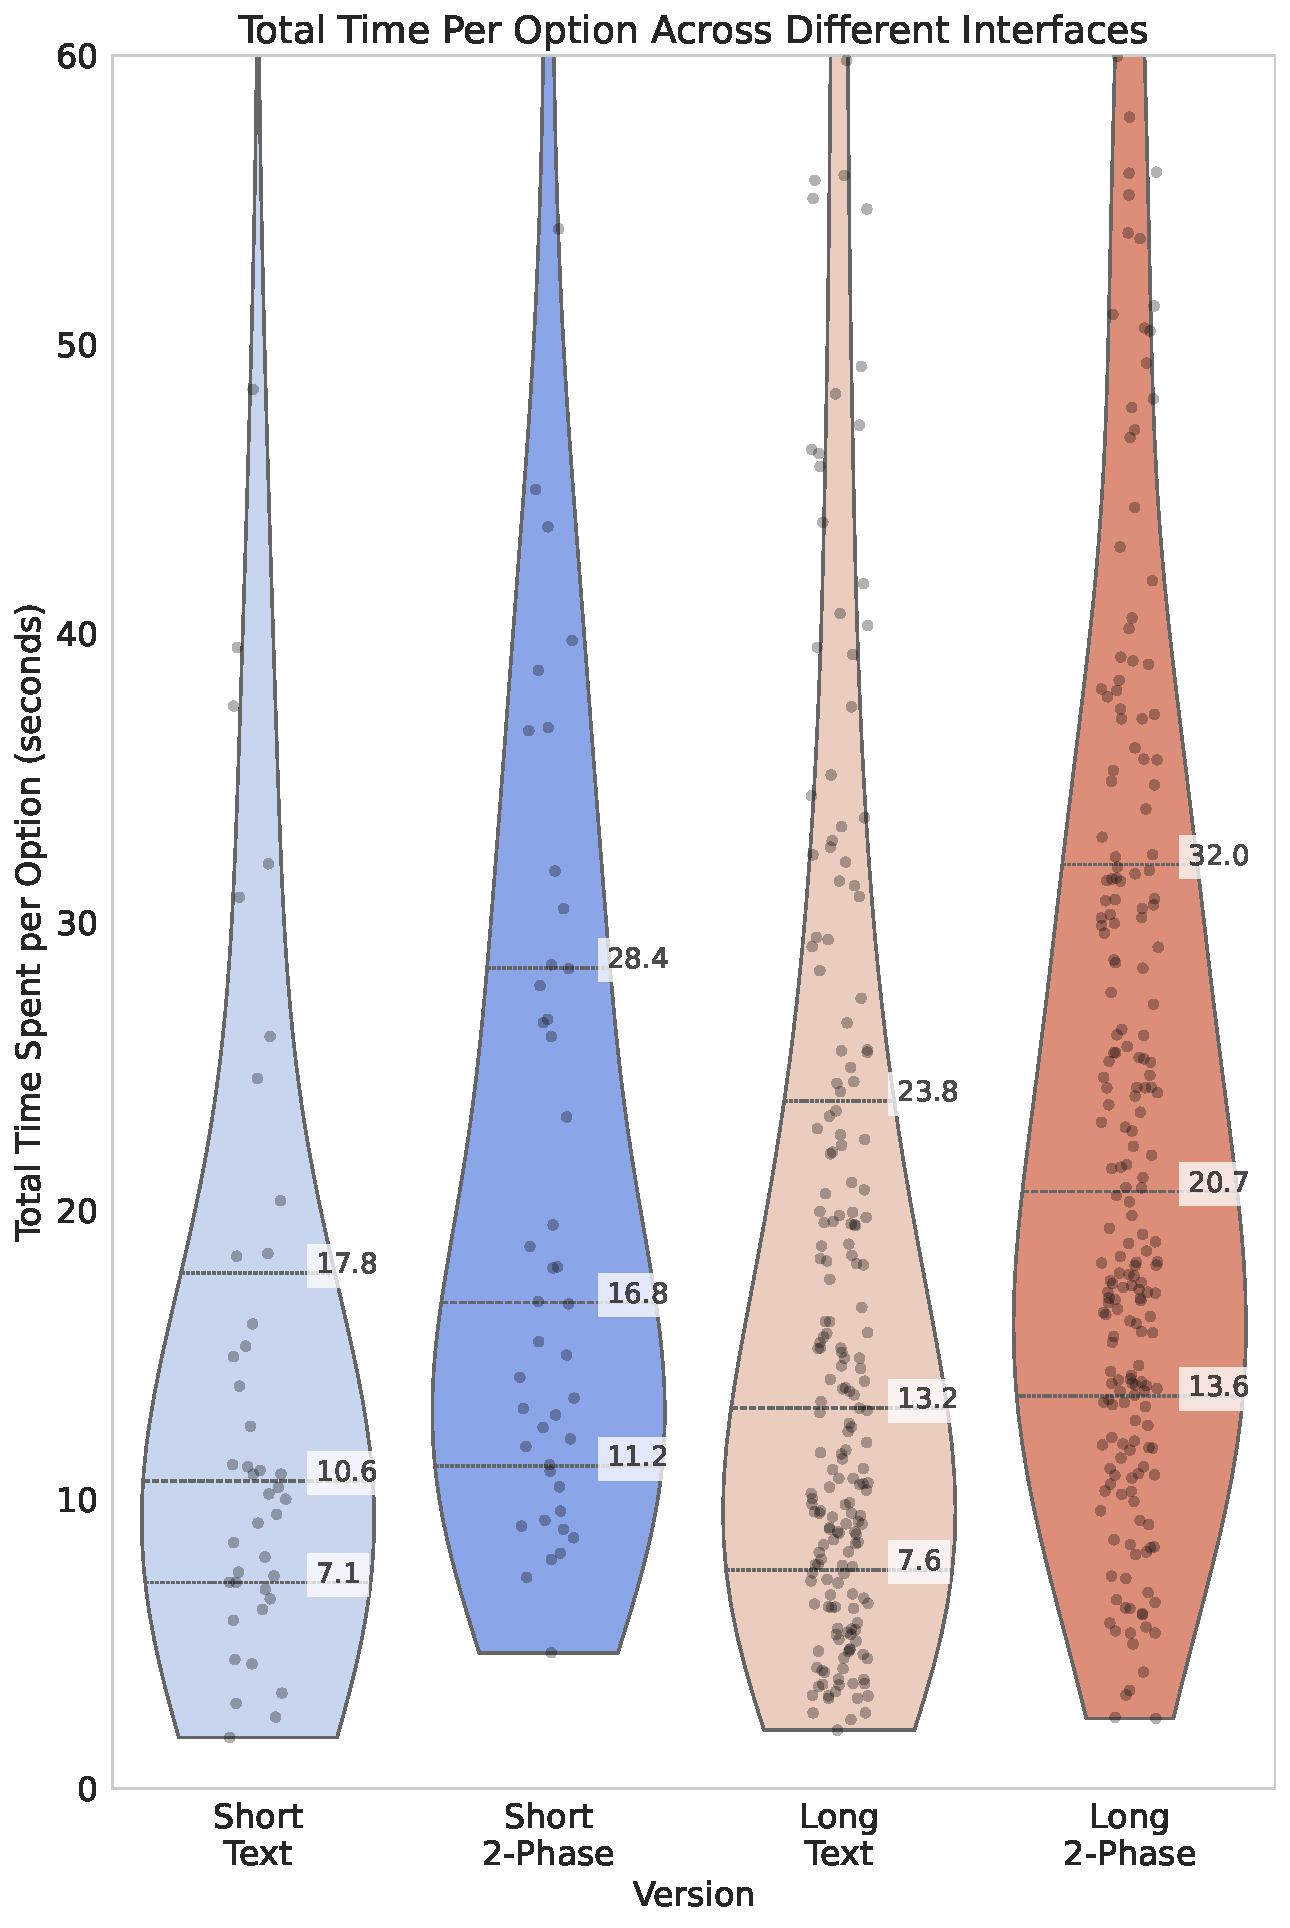
\includegraphics[width=\textwidth]{content/image/results/total_time_per_option.pdf}
                \captionsetup{width=0.87\textwidth}
                \caption{Total Time per option: We identified that two-phase interface skewed slightly higher than the text interface. This is reasonable since participants in these two conditions requires additional time to complete the organizing steps.}
                \label{fig:total_time}
            \end{subfigure}
            % \hfill
            \begin{subfigure}[b]{0.24\pdfpageheight}
                \centering
                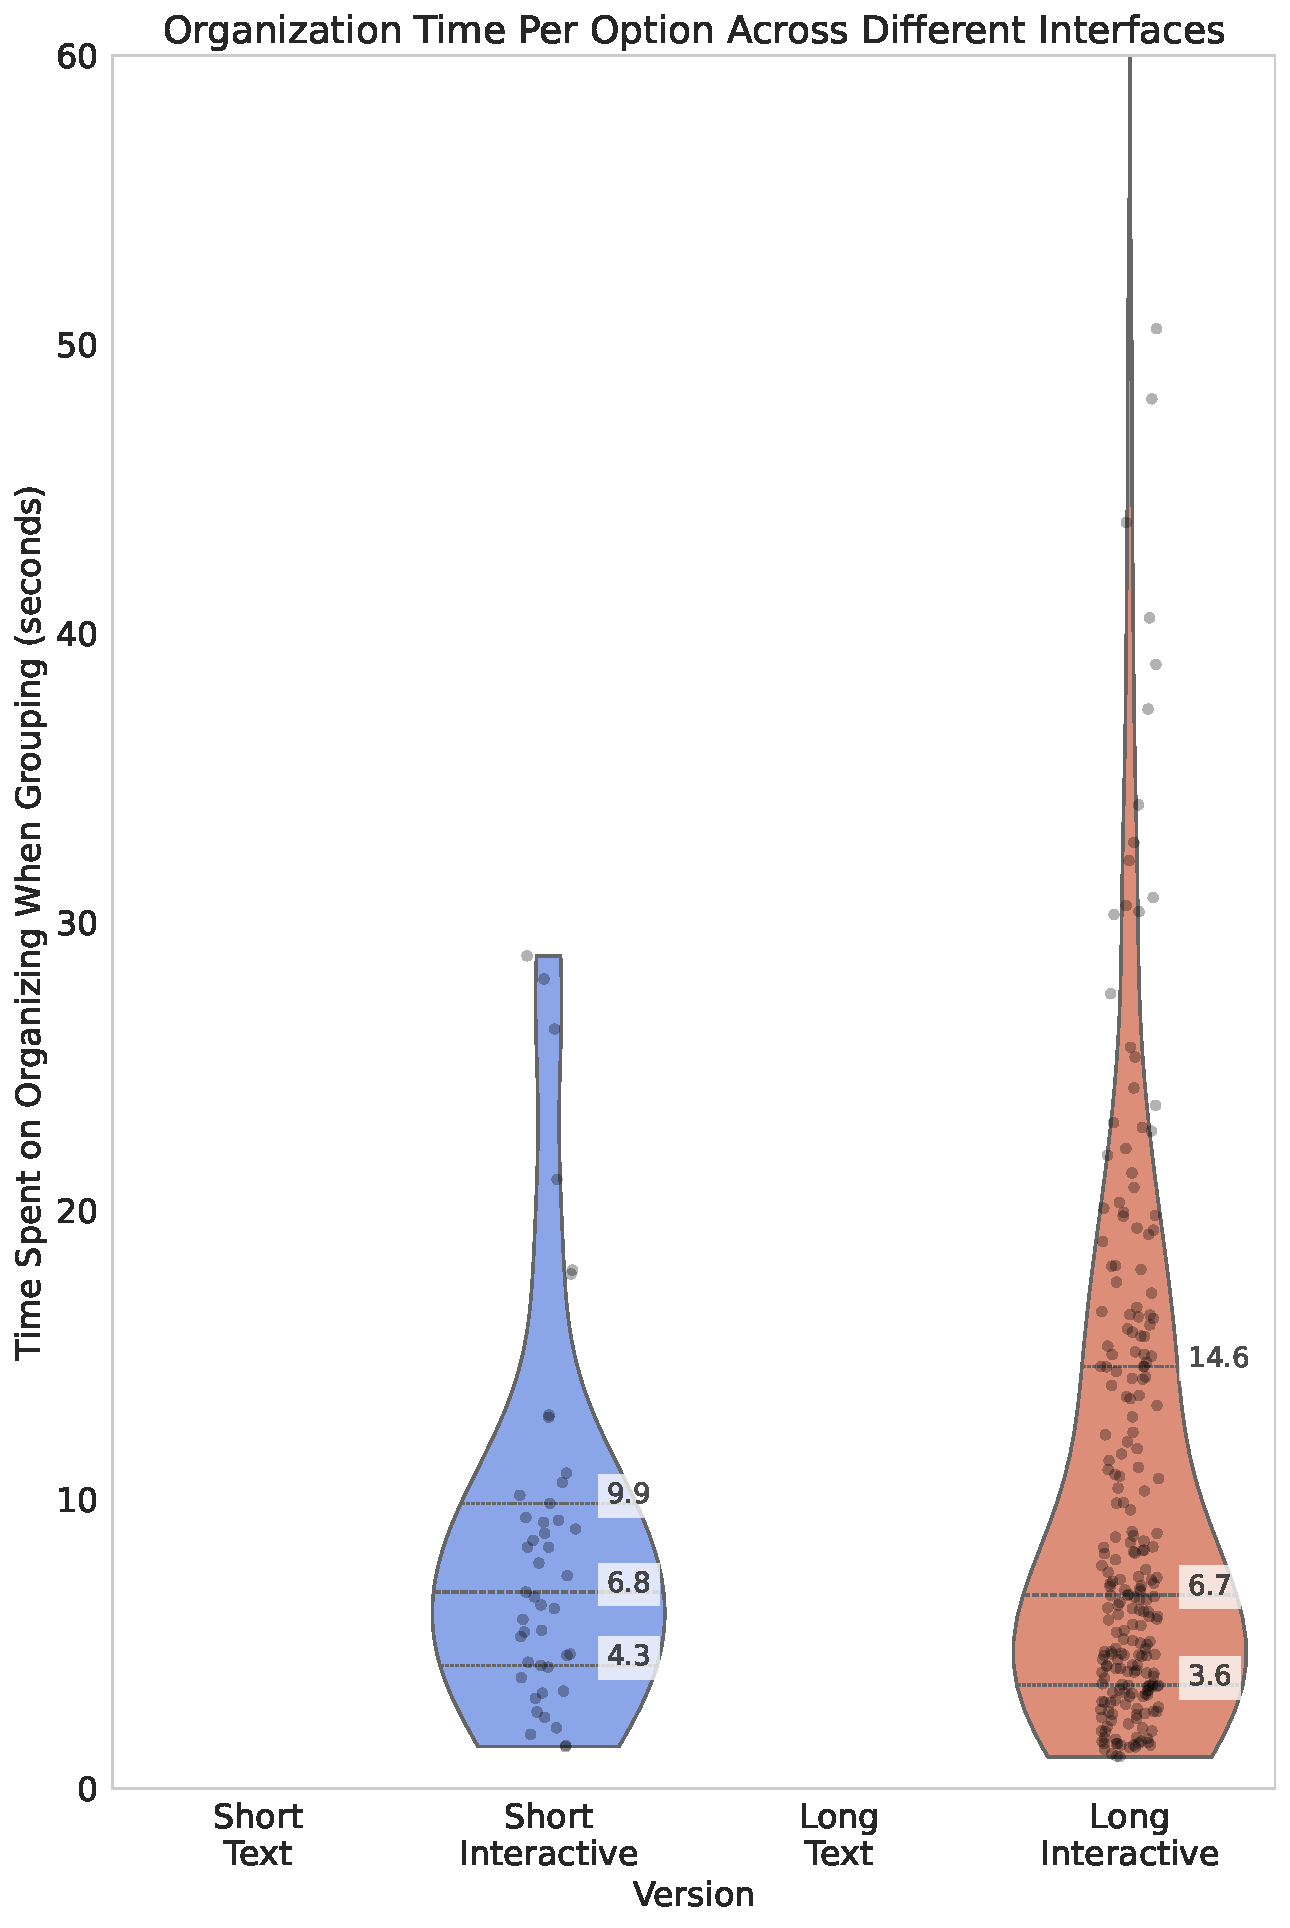
\includegraphics[width=\textwidth]{content/image/results/org_time_per_option.pdf}
                \captionsetup{width=0.87\textwidth}
                \caption{Organization Time per option: Since only two-phase interfaces has an organization phase, the other two experiment groups does not have any accumulated time.\vspace{25pt}}
                \label{fig:org_time}
            \end{subfigure}
            % \hfill
            \begin{subfigure}[b]{0.24\pdfpageheight}
                \centering
                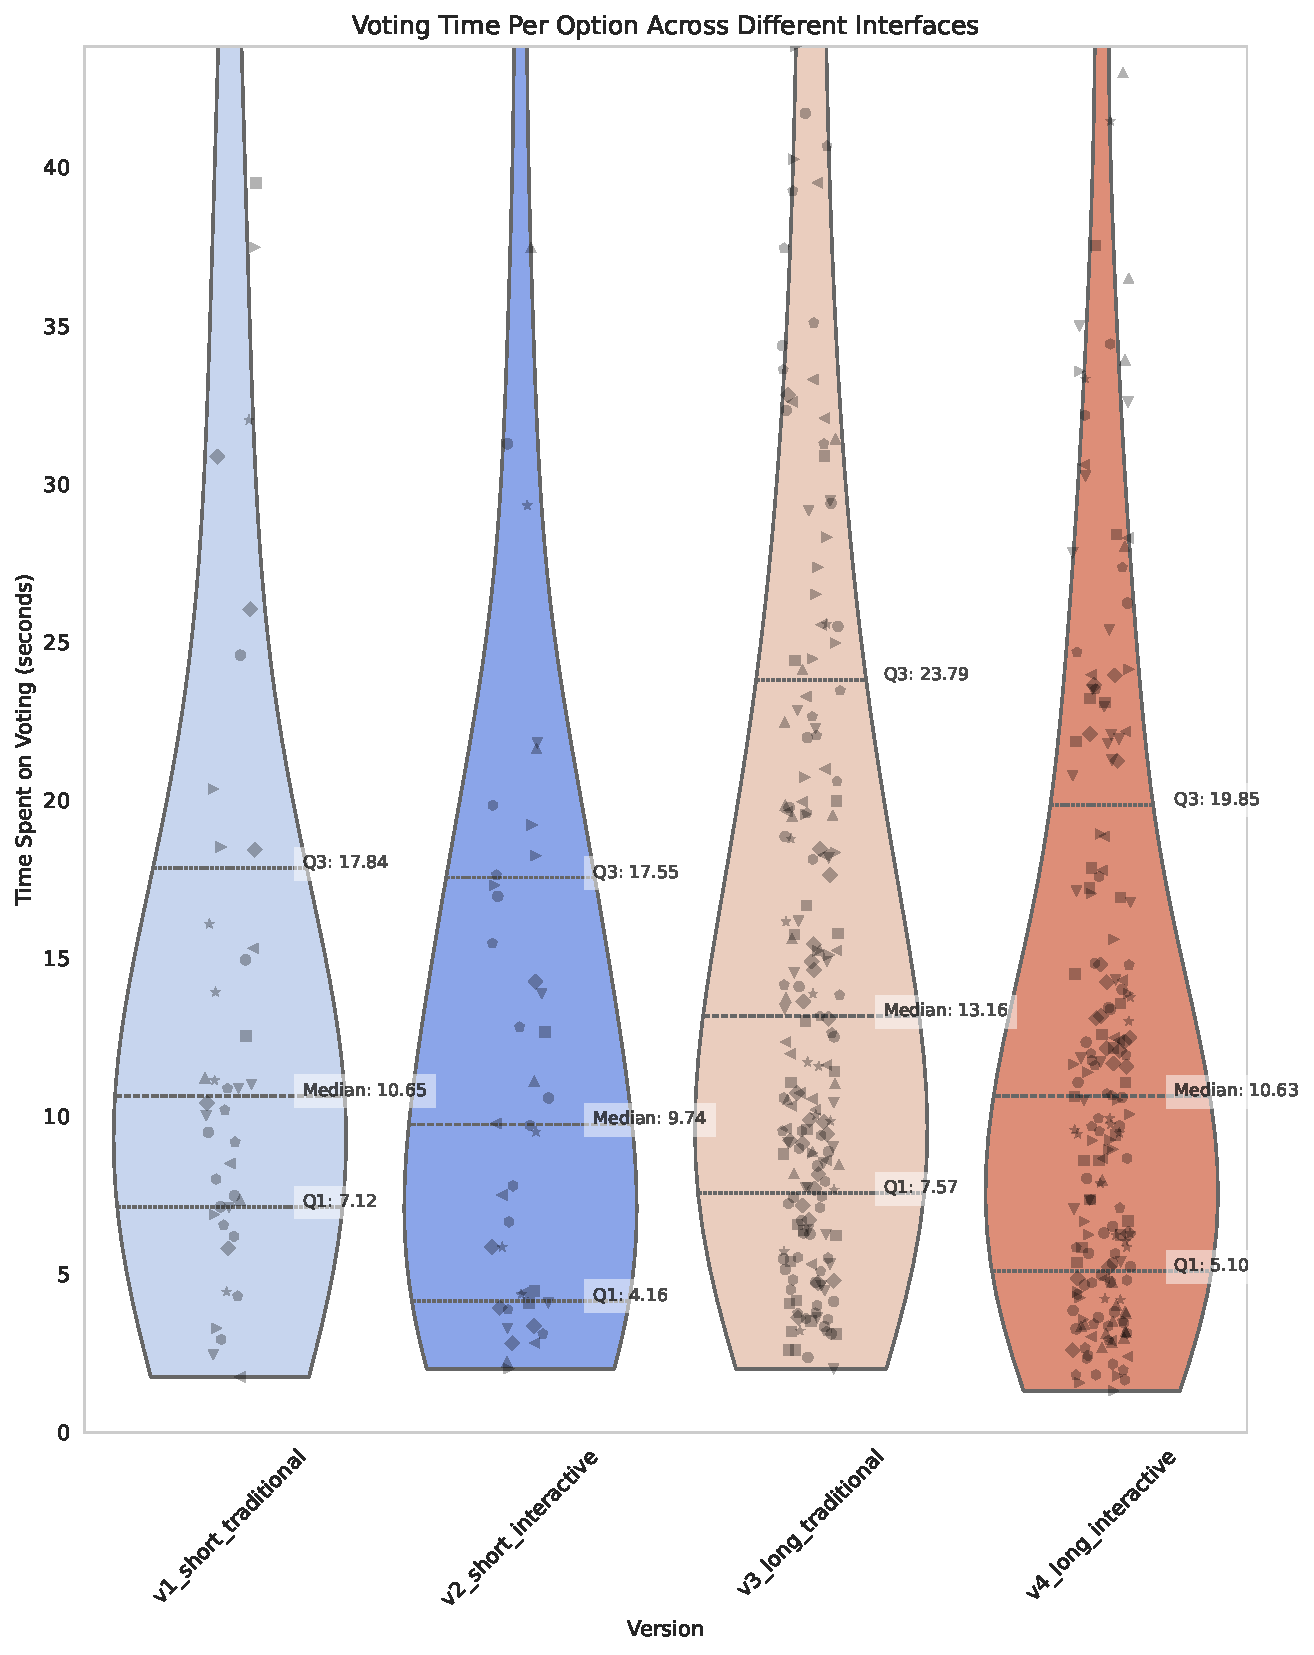
\includegraphics[width=\textwidth]{content/image/results/voting_time_per_option.pdf}
                \captionsetup{width=0.87\textwidth}
                \caption{Voting Time per option: We see a slight downward trend between the short QS, and a statistical faster voting time for the long two-phase interface.\vspace{25pt}}
                \label{fig:vote_time}
            \end{subfigure}
        \end{minipage}
    }
    \rotatebox{90}{%
        \begin{minipage}{\wd\savefig}
            
            \usebox{\savefig}
             \captionsetup{width=0.67\pdfpageheight}
            \caption{Time per option across all experiment conditions. In each of these violin plots, a dot represents the total time a participant spent on that option. Fig~\ref{fig:total_time} one dot represents the total time a person spent for one option. Figure~\ref{fig:org_time} and Figure~\ref{fig:vote_time} are decomposition of the total time.}
            \label{fig:time_per_option_full}
        \end{minipage}
    }
\end{figure}


\subsection{Time Spent per Option}
\label{sec:time_per_option}
Our first analysis focuses on understanding how much time participants spent per option across different stages and experiment conditions. Based on the QS system log, we can derive the following detailed logs of participant actions:~\textit{the option}  involved in the interaction,~\textit{the type of interaction} (such as updating a certain number of votes), and~\textit{the time} between this interaction and the previous one.

We aggregate all the time spent on each option as the total time spent for that option. Organization time covers both placing options into categories and the drag-and-drop time during the organization phase. Voting time strictly refers to the time participants took to update vote values for each option. To minimize noise, we intentionally drop all the time participants spent on the first option in the organization phase or voting phase. The goal is to exclude time spent on reading the prompt, forming their preference, or understanding the interface.

Figure~\ref{fig:time_per_option_full} each dot represents one option for one participant. Figure~\ref{fig:total_time} shows total time, figure~\ref{fig:org_time} shows organization time, and figure~\ref{fig:vote_time} shows voting time. The violin plot shows the distribution of the dots and the three horizontal lines represent the median, 25th percentile, and 75th percentile of the time spent for that interface. We limited the y-axis to 1 minute to improve visualization clarity.

Participants spent slightly more time per option on the two-phase interface than the text interface. A non-parametric Mann-Whitney U test showed a small effect size (long QS: $p<0.0000001$, Rank-biserial: $-0.304$, Cohen's d: $-0.030$; short QS: $p=0.01$, Rank-biserial: $-0.37$, Cohen's d: $-0.082$). This is expected as the two-phase interface has an additional step of organizing the options. We break down the total time spent into organization time and voting time in Figure~\ref{fig:org_time} and Figure~\ref{fig:vote_time}.

We observed minimal difference in organization time per option (Figure~\ref{fig:org_time}) between short and long surveys, as options are shown one at a time for drag-and-drop. In terms of the voting time (Figure~\ref{fig:vote_time}), participants spent significantly less time voting on the two-phase interface than on the text interface with a small effect size in the long QS ($U=24053$, $p<0.005$, Rank-biserial: $0.167$, Cohen's d: $0.017$), but not in the short survey ($p>0.4$, Power=$0.051$). This supports our hypothesis that the two-step design in the two-phase interface facilitates more efficient decision-making, especially in longer surveys.

\subsection{Budget and Voting Behaviors}
To further analyze participant behaviors, we break down the aggregated time from the previous analysis and examine fine-grain interactions. Specifically, we examine if there are differences among behavior across interfaces. As we outlined, credit scarcity might influence decision making.  Figure~\ref{fig:voting_all} plots the time of voting actions over the remainder of the participant's budget across the text and two-phase interface across all four groups. Each bar shows the number of actions accumulated across participants at specific percentages of remaining credits. A kernel density estimate (KDE) plot is provided to visualize the trends. We did not follow ~\textcite{quarfoot2017quadratic} in counting accumulated votes over time due to varying total times across individuals.

Comparing experiment groups, we see fewer differences in the short QS but different interaction distributions between the two interfaces in the long QS. Given the significant differences in voting time between the text and two-phase interface for the long QS, we focus on deciphering the voting action changes between these two conditions in this subsection.

\begin{figure}[ht]
    \centering
    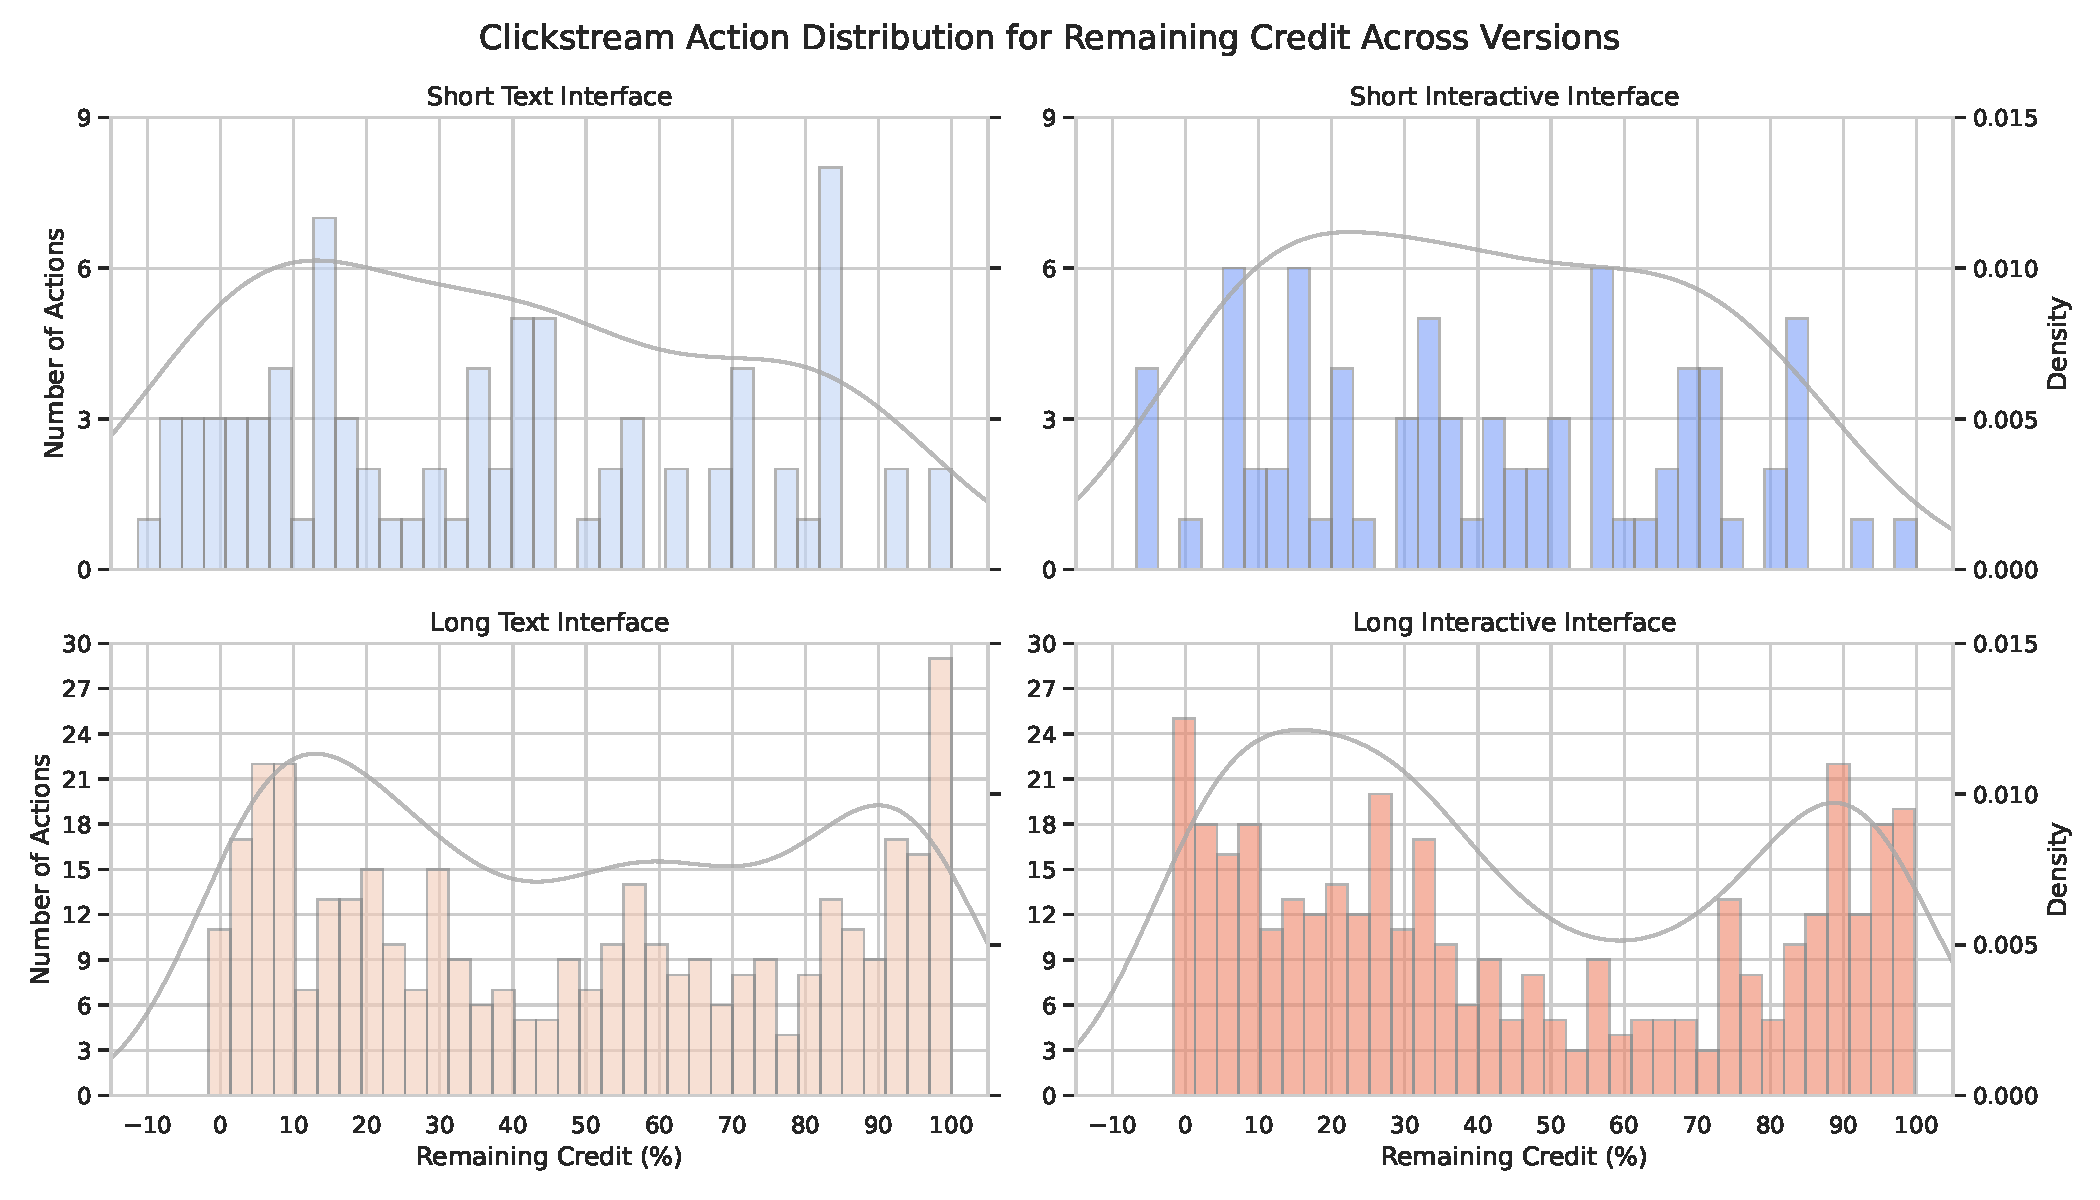
\includegraphics[width=\textwidth]{content/image/results/clickstream_action_distribution.pdf}
    \caption{This plot counts the number of voting actions when there are $x$ percentages of credits remaining. A KDE plot is provided to help better understand the action distribution.}
    \label{fig:voting_all}
\end{figure}

In Figure~\ref{fig:voting_all}, we see two distinct patterns between the short survey and the long survey in terms of participant behaviors. In long surveys, participants exhibited more actions both when the budget was abundant and when it began to run out. This pattern was more pronounced with the long two-phase interface. We further separated the behaviors where participants made large or small changes to the options, specifically for the long version. In Figure~\ref{fig:voting_v3_v4}, we define an adjustment of four or more votes as large, which we plotted in the first row of the figure. Adjustments of two or fewer votes are considered small, which is $10\%$ of the possible values one can choose among the maximum of 21 votes.

\begin{figure}[ht]
    \centering
    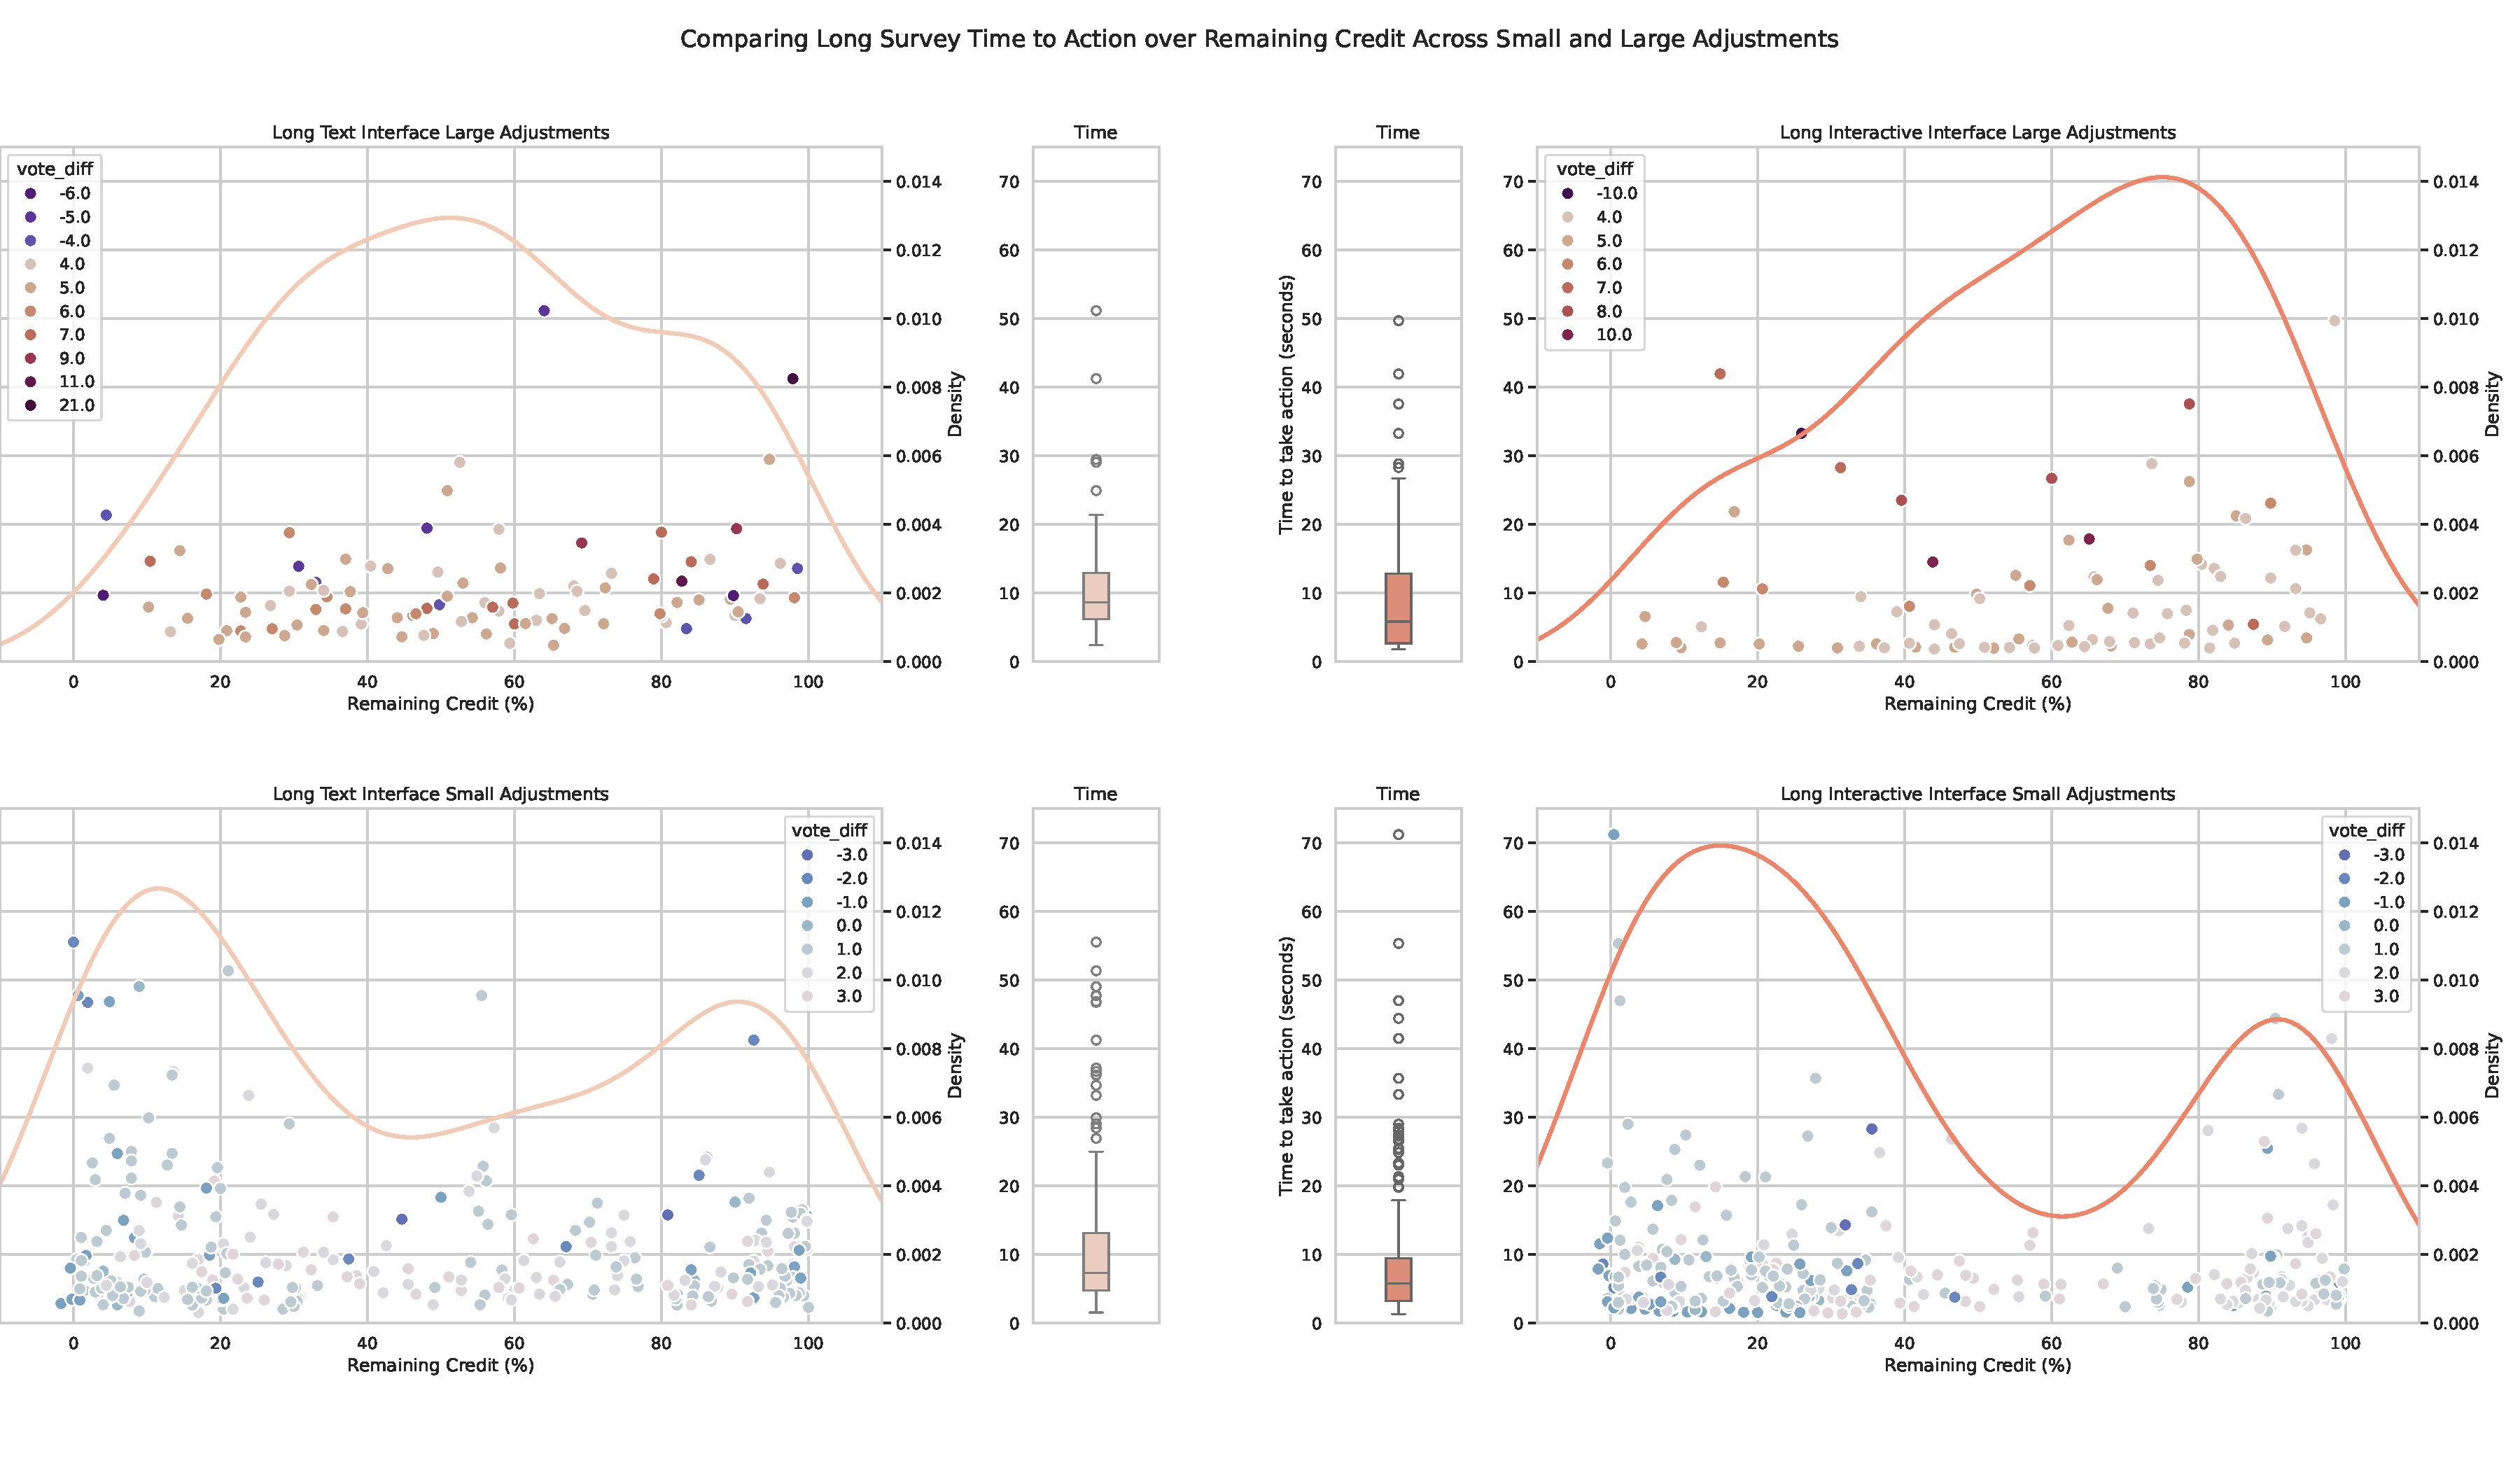
\includegraphics[width=\textwidth]{content/image/results/combined_density_plots.pdf}
    \caption{This plot further separates participants' interaction behavior based on the number of votes participants adjusted. We observed a bimodal interaction pattern across long QS when small vote adjustments are made.}
    \label{fig:voting_v3_v4}
\end{figure}

We plotted all actions against the time to complete them. Revisiting the KDE curve in the second row in Figure~\ref{fig:voting_all} and the curve of the second row in Figure~\ref{fig:voting_v3_v4} show a stronger bimodal distribution for small vote adjustments across interfaces. In fact, the bimodal distribution is more pronounced in the two-phase interface. This suggests that participants make small adjustments both at the beginning and toward the end of the QS. However, the two-phase interface shows more frequent and faster edits towards the end. Visually, dots are more clustered in the long two-phase interface for small vote adjustments compared to the long text interface. The Mann-Whitney U Test on the time spent on small vote adjustments showed significant differences ($U=13037$, $p<0.001$), with a small effect size (Rank-biserial: $0.227$, Cohen's d: $0.195$) and a power of $0.381$. Based on the KDE plots in the first row of Figure~\ref{fig:voting_v3_v4}, participants also made more large vote adjustments early on that spread more equally compared to the text interface. This indicates that participants had a clearer idea of how to distribute their credits across the options.

In interviews, five participants highlighted the importance of the interface's flexibility and their use of an incremental, iterative approach. All these participants used the two-phase interface. While this doesn't mean participants using the text interface didn't take an iterative approach, it highlights that the two-phase interface encouraged iterative and incremental updates. As one participant pointed out:

\begin{displayquote}
I like the fact that it remembers everything that you know.~\bracketellipsis that's very important is that it's an iterative process.\hfill\quoteby{S019 (LI)}
\end{displayquote}
% If you make a mistake, that you don't lose all the work that you've already done. so I think 

To summarize, participants spent more time on the two-phase interface compared to the text interface in both short and long surveys. Across the two-phase interfaces, organization time remained consistent. While voting time did not differ between interfaces for the short survey, participants voted more quickly on the two-phase interface in the long survey, confirming the hypothesis that the two-step design enhances decision-making efficiency. Voting behaviors indicated more frequent actions when the budget was abundant and nearly exhausted, particularly in the long two-phase interface. Additionally, the analysis revealed more frequent and faster small vote adjustments towards the end of the QS in the two-phase interface, demonstrating an iterative and incremental approach. 

% content removed in discussion should make sure are in this section
%  , as reflected in slightly faster voting times

% This suggests that participants in the interactive interface are more likely to make larger adjustments to their votes. This is consistent with the observation that participants in the interactive interface spent more time on voting actions in the long survey. We also see a cluster of voting actions in the bottom left corner of the interactive interface for small vote adjustments. This suggests that participants in the interactive interface are more likely to make small adjustments when their budget is running low. This is consistent with the observation that participants in the interactive interface spent less time on voting actions in the long survey.
% First, surface the bimodal action distribution in both plots, with a even stronger signal for long interactive interface participants. Second, the plot demonstrated a clear cluster of voting actions in the bottom left corner of the interactive interface for small vote adjustments. In other words, participants made much smaller but more rapid adjustments when their budgets were running low. Second, larger adjustments are made when the participants have more options comparing the two plots on the first row. We interpret this behavior as participants in the interactive interface have constructed a clearer image of option preferences and, hence, have the ability to take larger strides in allotting their budget and deciding the number of votes at the beginning of the survey. Toward the end, participants using the interactive interface are then making fine-tuned adjustments to ensure that their preferences are reflected in their submissions.

% add qualitative support


% Ti-Chung Cheng: So what elements of the software interface do you dislike, or like the most, if any, when expressing your preferences on responding to societal issues?
% S009: Hmm! What I like the most actually, probably the sorting function. I think that it really helped me organize my thoughts really, clearly, in terms of what I would dislike the most. really, not that much. I would say. yeah, also, like how we could categorize it, like even within the voting stage rather than just at the categorization stage. 

% Ti-Chung Cheng: Can you tell me a little bit more about the screen? How did the vertical screen help you?
% S037: I think because it helps the layout of, because it's like a long 3 bar. So it's easier for you to to drag and drop, and you can actually sort it, judging by the votes. But I do not do that. But I think this layout is could be helpful in that aspect.


